%AUTHOR:Michael Kramer
Because the symbol-timing requires a feed-back loop, you will
have to simulate the DLL on a sample by sample basis in \matlab.

Using an square wave of period $32$ samples as input, simulate
the DLL system shown in Figure \ref{fig: dll}.  Your input
should be several hundred periods long and you will want to
set the early/late accumulations threshold to $1.0$ to start with 
(How will a different threshold level affect the locking ability of the DLL?)

The figures below show the matched filter output and the corresponding
sampling times (indicated by the impulses) for the beginning 
of the input, before the DLL has locked on, as well as after
1000 samples (about 63 symbols worth), when symbol timing lock has
been achieved.  Note the location of the ``on-time'' sampling times
with respect to the peaks of the averaging filter output
for each case.
 
\begin{figure}[ht]
   \begin{center}
      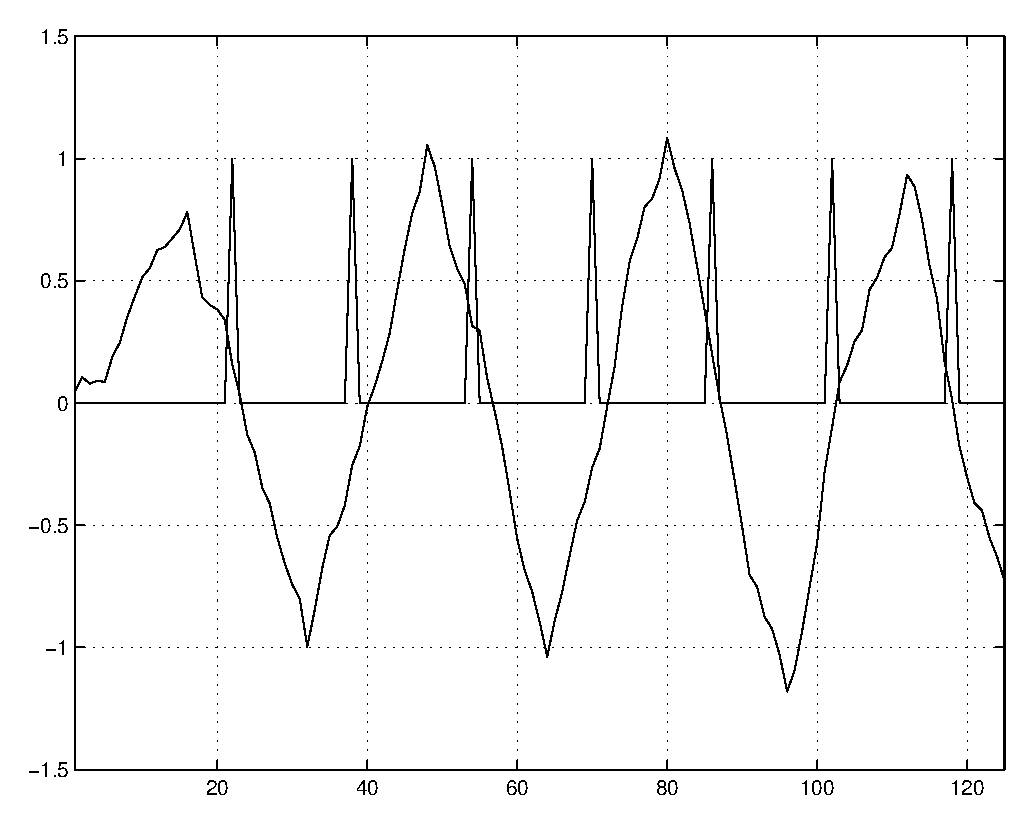
\epsfig{file=non_locked_dll.eps,width=6cm}
      \caption{Symbol sampling before DLL lock.}
      \label{fig: dll_before_lock}
   \end{center}
\end{figure}

\begin{figure}[ht]
   \begin{center}
      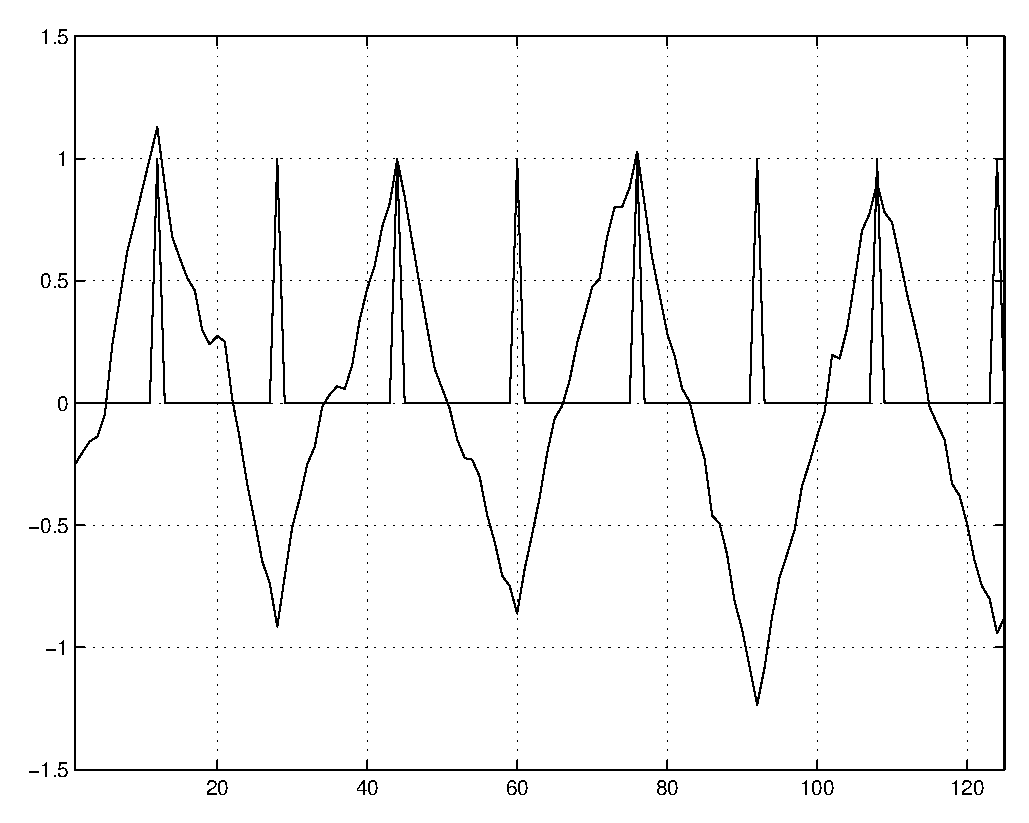
\epsfig{file=locked_dll.eps,width=6cm}
      \caption{Symbol sampling after DLL lock.}
      \label{fig: dll_after_lock}
   \end{center}
\end{figure}

